% ============================================================================
%  CLDB: Continual Reinforcement Learning for Autonomous Index Selection
%  under Workload Drift
%
%  Compile:  pdflatex main && bibtex main && pdflatex main && pdflatex main
%  (Requires: amsmath, amssymb, booktabs, graphicx, natbib, algorithm,
%   algpseudocode, tikz, hyperref. Tested with a standard TeX Live install.)
% ============================================================================
\documentclass[10pt,twocolumn]{article}

\usepackage[margin=0.75in]{geometry}
\usepackage{amsmath,amssymb,amsthm}
\usepackage{booktabs}
\usepackage{graphicx}
\usepackage{algorithm}
\usepackage{algpseudocode}
\usepackage{tikz}
\usetikzlibrary{arrows.meta,positioning,fit,backgrounds}
\usepackage[numbers,sort&compress]{natbib}
\usepackage[hidelinks]{hyperref}
\usepackage{xcolor}
\usepackage{caption}
\captionsetup{font=small}
\usepackage{balance}

\newtheorem{proposition}{Proposition}
\newtheorem{lemma}{Lemma}
\newtheorem{definition}{Definition}
\newtheorem{remark}{Remark}
\newcommand{\R}{\mathbb{R}}
\newcommand{\E}{\mathbb{E}}
\newcommand{\KL}{\mathrm{KL}}
\newcommand{\State}{\mathcal{S}}
\newcommand{\Action}{\mathcal{A}}
\newcommand{\loss}{\mathcal{L}}
\newcommand{\Fforget}{\mathcal{F}}

\title{\vspace{-1.2em}\textbf{CLDB: Continual Reinforcement Learning for\\
Autonomous Index Selection under Workload Drift}\vspace{-0.4em}}

\author{
Ibhan Mukherjee\\
\texttt{ibhan@example.com}
\and
Anonymous Co-Author(s)
}

\date{}

\begin{document}
\maketitle

\begin{abstract}
Autonomous index advisors based on machine learning, and the emerging class of
reinforcement-learning (RL) advisors, are trained once and then deployed under
the implicit assumption that the query workload is \emph{stationary}. In
production, workloads are anything but stationary: the query mix drifts across
daily, weekly, and seasonal phases, so an advisor that was optimal last month is
often sub-optimal today. Keeping such an advisor current today requires
\emph{periodic offline retraining}, which is expensive and disrupts service; the
obvious alternative---naively fine-tuning the deployed policy on the new
workload---causes \emph{catastrophic forgetting} of the workload phases the
advisor already mastered. We formulate index selection as a \emph{continual
reinforcement-learning} problem and introduce \textbf{CLDB}, an online
index-selection agent that must solve a non-stationary sequence of workload
phases without retraining from scratch and without forgetting. CLDB couples
(\(i\)) an off-policy deep Q-network whose state includes the current
index configuration, (\(ii\)) \emph{drift-triggered elastic weight
consolidation} that anchors the policy only when workload drift is detected,
(\(iii\)) a \emph{database-aware prioritized replay} buffer whose priorities
combine latency impact with workload rarity and are refined by TD errors, and
(\(iv\)) structural action masking that prevents unsafe schema changes. We build
a reproducible cost-model benchmark of conflicting workload phases and evaluate
with the standard continual-learning metrics ACC, BWT, FWT and forgetting. Across
eight seeds, an online agent that learns without rehearsal \emph{catastrophically
forgets}: its forgetting is \(\mathcal{F}=0.20\pm0.03\) and its backward transfer
is strongly negative (\(\mathrm{BWT}=-0.20\)), both significantly worse than a
replay-based agent ($p<0.05$ paired $t$-test). Restoring a replay buffer reduces
forgetting to \(\mathcal{F}\approx0.10\text{--}0.13\). Drift-triggered EWC moves
forgetting in the expected direction but its additional contribution over replay
is not statistically significant in this benchmark---an honest negative result we
report. All learning agents beat the static KEEP and RANDOM baselines and
\emph{match} a structural CREATE heuristic on reward while remaining adaptive. We
give a full mathematical formulation, a theoretical analysis of the EWC
objective, the value-network Fisher estimator, the prioritized-replay gradient
and the consolidation cost, an open-source implementation, and a candid discussion
of the gap between this prototype and a production-grade study.

\end{abstract}

\section{Introduction}

Modern database management systems are increasingly \emph{self-driving}: they
observe their own workload and act on it without human intervention
\citep{pavlo2017selfdriving}. Physical design---in particular, choosing which
secondary indexes to create and drop---is one of the highest-leverage knobs in
such a system, because indexes can change query latency by orders of magnitude.
Classical index advisors formulate this as a what-if optimization problem over a
fixed, known workload and solve it with greedy search or integer programming
\citep{chaudhuri1997autoadmin,valentin2000db2advisor,zilio2004db2design}. These
advisors are \emph{offline} and \emph{assume a stationary workload}: the workload
is collected, the advisor is run, indexes are materialized, and the loop stops.

Recent work replaces the hand-designed search with learned models, including
learned cost estimators \citep{marcus2019learnedcost}, learned cardinality
estimators \citep{kipf2019learnedcardinalities}, learned index structures
\citep{kraska2018case}, and learned query optimizers such as Bao
\citep{marcus2021bao}. A parallel line applies reinforcement learning (RL) to
physical design, training an agent to propose index actions and rewarding it with
observed latency improvements. All of these systems share the same hidden
assumption as their classical predecessors: \emph{the workload used to train the
model is the workload that will be served at deployment time.}

Production workloads violate this assumption. A transactional system looks very
different at 9~a.m.\ (short, selective, point lookups on the \texttt{orders}
table) than at 2~a.m.\ (long analytical scans over the same table); retail
systems shift with campaigns and seasons; and schemas and access patterns evolve
over months. We call such a temporally evolving workload a \emph{workload drift},
and the periods over which the workload distribution is approximately stationary
\emph{workload phases}. When the workload drifts, a deployed advisor faces a
dilemma:
\begin{enumerate}
  \item \textbf{Offline retraining} from scratch on the new workload is
    expensive, requires collecting and labelling a batch of queries, and
    disrupts the service; it also discards knowledge of previous phases that may
    return.
  \item \textbf{Online fine-tuning} on recent queries is cheap and
    non-disruptive, but naively updating the parameters on the new phase causes
    \emph{catastrophic forgetting} \citep{mccloskey1989catastrophic}: the agent
    rapidly loses the ability to optimize the phases it previously mastered,
    which is exactly the situation when the workload later returns to a previous
    phase.
\end{enumerate}
This is the continual-learning trilemma---\emph{adapt}, \emph{retain}, and
\emph{stay cheap/online}---and existing index advisors address at most two of the
three.

\paragraph{Approach.}
We argue that autonomous index selection should be posed not as a single-task RL
problem but as a \emph{continual reinforcement-learning} problem
\citep{khetarpal2022continual}. We therefore introduce \textbf{CLDB}, an online
index-selection agent that learns an unbounded sequence of non-stationary
workload phases from live query feedback. CLDB makes four design contributions,
all of which are implemented end-to-end:
\begin{itemize}
  \item \textbf{Index-aware off-policy DQN.} The agent is a deep Q-network
    \citep{mnih2015dqn} with a target network. Crucially, the state includes the
    \emph{current index configuration} (number of active indexes, whether the
    current predicate is covered, and remaining budget), making the process a
    genuine Markov decision process rather than a contextual bandit: creating an
    index has a one-time cost and a recurring benefit, and dropping it is a
    decision that depends on the accumulated index state.
  \item \textbf{Drift-triggered EWC.} Instead of consolidating at fixed task
    boundaries (which are unknown online), CLDB computes the elastic weight
    consolidation penalty \citep{kirkpatrick2017ewc} only when a drift detector
    \citep{gama2014drift} fires. We analyze the cost of this event-driven rule
    relative to boundary-based consolidation (Lemma~\ref{lem:consolidation}).
  \item \textbf{Database-aware prioritized replay.} The replay buffer
    prioritizes experiences by their \emph{database impact}---absolute latency
    reward times workload rarity---and refines those priorities with absolute TD
    errors, combining the anti-forgetting effect of experience replay
    \citep{rolnick2019replay} with the sample efficiency of prioritized replay
    \citep{schaul2016prioritized}.
  \item \textbf{Safety-constrained exploration.} A structural action mask forbids
    \texttt{CREATE\_INDEX} without predicate columns and \texttt{DROP\_INDEX}
    without an existing index, so exploration can never propose an unsafe schema
    change.
\end{itemize}

\paragraph{Research questions.}
CLDB is designed to answer the following question and its refinements:
\begin{quote}
\emph{Can a reinforcement-learning index-selection policy continually acquire new
workload phases from live query feedback---while retaining competence on
previously seen phases---without offline retraining or blocking query
execution?}
\end{quote}
Concretely we ask: \textbf{(RQ1)} does the agent retain earlier phases better
than naive online fine-tuning? \textbf{(RQ2)} which mechanism drives retention,
replay or EWC? \textbf{(RQ3)} does database-aware prioritization beat uniform
replay? \textbf{(RQ4)} does action masking help or hurt? \textbf{(RQ5)} can
adaptation happen online at bounded cost?

\paragraph{Contributions.}
\begin{enumerate}
  \item We give the first formulation of index selection as a continual
    reinforcement-learning problem with an index-aware state, and we provide a
    reproducible \emph{cost-model benchmark} of conflicting workload phases that
    induces genuine catastrophic forgetting (Section~\ref{sec:problem},
    Section~\ref{sec:experiments}).
  \item We design and implement a complete agent---drift-triggered EWC,
    database-aware prioritized replay, and safety masking---together with an
    online pipeline that satisfies the non-blocking requirement
    (Section~\ref{sec:method}).
  \item We provide a theoretical analysis: the EWC objective as a Laplace
    posterior approximation (Proposition~\ref{prop:ewc}), the value-network
    Fisher estimator (Proposition~\ref{prop:fisher}), the unbiasedness of the
    prioritized-replay gradient (Proposition~\ref{prop:per}), and the
    consolidation-cost advantage of drift triggering
    (Lemma~\ref{lem:consolidation}) (Section~\ref{sec:theory}).
  \item We evaluate against static, random and heuristic baselines and against
    ablations (no EWC, no replay) using the standard continual-learning metrics
    ACC, BWT, FWT and forgetting \citep{lopezpaz2017gem}, with eight seeds and
    paired significance tests (Section~\ref{sec:results}). The central,
    statistically significant finding is that \emph{rehearsal} (replay) is the
    ingredient that prevents catastrophic forgetting; EWC's incremental benefit is
    smaller and, in this benchmark, not significant---a result we report and
    analyze rather than hide.
\end{enumerate}

\paragraph{Organization.}
Section~\ref{sec:related} reviews related work. Section~\ref{sec:problem} gives
the mathematical formulation. Section~\ref{sec:method} describes CLDB.
Section~\ref{sec:theory} develops the theory. Sections~\ref{sec:experiments}
and~\ref{sec:results} present the setup and results.
Section~\ref{sec:discussion} discusses limitations and threats to validity, and
Section~\ref{sec:conclusion} concludes.

\section{Related Work}
\label{sec:related}

\paragraph{Classical index advisors.}
Index selection as an optimization problem dates to the AutoAdmin project
\citep{chaudhuri1997autoadmin}, which searches over candidate index
configurations using a what-if optimizer. The DB2 Advisor
\citep{valentin2000db2advisor} and the DB2 Design Advisor
\citep{zilio2004db2design} extended this to multiple design structures and budget
constraints. These systems assume a fixed workload, solve an offline
optimization problem, and are re-run manually when the workload changes.

\paragraph{Learned database components.}
Machine learning now pervades the database internals. Learned index structures
\citep{kraska2018case} replace B-trees with models; learned cardinality
estimators \citep{kipf2019learnedcardinalities} and learned cost models
\citep{marcus2019learnedcost} improve plan costing; and Bao \citep{marcus2021bao}
learns to steer the query optimizer at plan time. Each of these components is
trained offline on a corpus and then frozen; none addresses the question of how a
\emph{deployed} model should keep learning as the workload evolves.

\paragraph{Reinforcement learning for physical design.}
A growing body of work casts physical design as an RL problem. In the bandit
setting, an agent chooses configuration actions (create/drop an index,
materialize a view) and receives a latency-based reward. Such approaches are
attractive because they avoid an explicit what-if oracle, but they inherit the
stationarity assumption: the agent is trained and evaluated on a fixed workload
distribution, and a distribution shift degrades performance. To the best of our
knowledge, CLDB is the first to treat index selection as a \emph{continual} RL
problem and to combine continual-learning machinery with an index-aware RL
formulation.

\paragraph{Continual learning.}
Continual learning (CL) seeks to learn a sequence of tasks without forgetting.
Regularization methods constrain updates to protect parameters important for
previous tasks; elastic weight consolidation (EWC) \citep{kirkpatrick2017ewc}
does so using the Fisher information matrix, while learning-without-forgetting
\citep{li2017lwf} distils the old model's outputs. Rehearsal methods store and
replay a subset of past data, either uniformly \citep{rolnick2019replay} or
through gradient episodic memory \citep{lopezpaz2017gem}, which projects
gradients to avoid increasing the loss on buffered examples. The last two
references also define the ACC/BWT/FWT metrics we adopt. Our contribution is not
a new CL algorithm but the \emph{combination} of these ideas with a
database-specific priority signal and a drift-triggered consolidation rule taken
from the concept-drift literature \citep{gama2014drift}.

\paragraph{Continual and non-stationary RL.}
Reinforcement learning under non-stationarity is surveyed by
\citet{khetarpal2022continual}. Deep RL relies on experience replay and target
networks \citep{mnih2015dqn,lillicrap2016ddpg}; prioritized replay
\citep{schaul2016prioritized} reweights transitions by TD error with importance
sampling; double Q-learning \citep{vanhasselt2016double} reduces overestimation.
Applying these ideas to a stream of \emph{conflicting} tasks is exactly the
continual-RL setting, and EWC was originally demonstrated on sequential Atari
games \citep{kirkpatrick2017ewc}. CLDB instantiates that setting for index
selection.

\paragraph{Gap.}
Existing index advisors are stationary; existing learned-DB components are frozen
after training; and existing continual-learning methods are demonstrated on
generic benchmarks rather than database tuning. CLDB sits at the intersection of
the three: a \emph{continual}, \emph{index-aware}, \emph{safety-constrained}
reinforcement-learning advisor, evaluated with continual-learning metrics on a
reproducible workload-drift benchmark.

\section{Problem Formulation}
\label{sec:problem}

\subsection{Notation and the index-selection setting}
Let \(q\) denote a SQL query and \(I\) a set of secondary indexes, where each
element of \(I\) is a set of columns. Query \(q\) has a set of
\emph{predicate columns} \(\pi(q)\) (the columns referenced in its
\textsc{where}/\textsc{on} clauses), extracted by a SQL parser. For a
(column, index) coverage relation we write \(\pi(q) \sqsubseteq I\) if some index
in \(I\) contains all the predicate columns of \(q\).

We model the operating cost of serving \(q\) under index configuration \(I\) as
\begin{equation}
  C(q, I) = L(q, I) + \rho\,|I|,
  \label{eq:cost}
\end{equation}
where \(L(q,I)\) is the query latency and \(\rho\,|I|\) is an amortized
maintenance/space cost charged per index per unit time. In our benchmark
\(L(q,I)\) takes one of two values depending on whether the predicate is
\emph{covered} \emph{and} \emph{selective}; in a real deployment \(L\) is
measured directly. Let \(\operatorname{sel}(c, p)\) denote the selectivity of
column \(c\) in phase \(p\) (a high-selectivity predicate benefits from an index;
a low-selectivity one does not). Then
\begin{equation}
  L(q,I) =
  \begin{cases}
    \ell_{\text{low}} & \text{if } \pi(q)\sqsubseteq I \text{ and } \pi(q)
      \text{ is selective for the phase,}\\
    \ell_{\text{high}} & \text{otherwise,}
  \end{cases}
  \label{eq:latency}
\end{equation}
with \(\ell_{\text{low}} \ll \ell_{\text{high}}\). Creating an index incurs a
one-time build cost \(\kappa\).

\subsection{The index-selection MDP}
We formulate a per-query decision problem as a Markov decision process (MDP)
\(M = (\State, \Action, P, R, \gamma)\).

\paragraph{State.}
At step \(t\) the state concatenates four components,
\begin{equation}
  s_t = \big[\,\underbrace{\phi(q_t)}_{\in\R^{74}} \;\|\;
   \underbrace{e(q_t)}_{\in\R^{384}} \;\|\;
   \underbrace{c_t}_{\in\R^{3}} \;\|\;
   \underbrace{\iota(I_t)}_{\in\R^{3}}\,\big] \in \R^{464},
  \label{eq:state}
\end{equation}
where \(\phi(q)\) is a structural feature vector (join count, presence of
\textsc{group by}/\textsc{order by}, estimated cardinality, and a hashed
bag-of-words over tables and predicate columns), \(e(q)\) is a semantic
embedding of the query text, \(c_t\) are normalized workload-context statistics
(phase index, progress, index-utilization), and \(\iota(I_t)\) is the
\emph{index-configuration state}
\begin{equation}
  \iota(I) = \big[\,|I|/B,\;\;
    \mathbb{1}[\pi(q)\sqsubseteq I],\;\;
    \max(0,(B-|I|)/B)\,\big],
  \label{eq:indexstate}
\end{equation}
with index budget \(B\). The inclusion of \(\iota\) is what makes the problem a
\emph{control} problem over index configurations rather than a one-shot
classification: the same query has different optimal actions depending on which
indexes are already present.

\paragraph{Action.}
\(\Action = \{0,1,2\}\) corresponding to
\textsc{keep}, \textsc{create\_index} (on \(\pi(q_t)\)), and
\textsc{drop\_index} (on \(\pi(q_t)\)). A structural mask
\(\mu(s_t)\in\{0,1\}^{|\Action|}\) disables infeasible actions:
\(\textsc{create}\) is allowed only if \(\pi(q_t)\neq\emptyset\) and
\(|I_t|<B\); \(\textsc{drop}\) is allowed only if an index equal to
\(\pi(q_t)\) is active.

\paragraph{Transition.}
Given \(a_t\), the index configuration updates deterministically,
\begin{equation}
  I_{t+1} =
  \begin{cases}
    I_t \cup \{\pi(q_t)\} & a_t=\textsc{create},\\
    I_t \setminus \{\pi(q_t)\} & a_t=\textsc{drop},\\
    I_t & a_t=\textsc{keep},
  \end{cases}
  \label{eq:transition}
\end{equation}
and the next query \(q_{t+1}\) is drawn from the current phase distribution.

\paragraph{Reward.}
The reward is the negative operating cost after the action, minus the build cost,
\begin{equation}
  R(s_t,a_t) = -\Big(L(q_t, I_{t+1}) + \rho|I_{t+1}|\Big)
              - \kappa\,\mathbb{1}[a_t=\textsc{create}].
  \label{eq:reward}
\end{equation}
Equation~\eqref{eq:reward} is dense, bounded, and directly tied to the quantity
an operator cares about; it makes \textsc{create} a temporally extended decision
(pay now, benefit later) and therefore justifies a discount factor \(\gamma<1\)
and a value function.

\paragraph{Objective.}
The agent seeks a policy \(\pi_\theta:\State\to\Delta(\Action)\) maximizing the
discounted return
\begin{equation}
  J(\theta) = \E_{\tau\sim\pi_\theta}\Big[\textstyle\sum_{t\ge0}\gamma^t R(s_t,a_t)\Big].
  \label{eq:objective}
\end{equation}
The optimal action-value function satisfies the Bellman optimality equation
\(Q^\star(s,a) = \E_{s'}[R(s,a) + \gamma\max_{a'} Q^\star(s',a')]\), and
\(\pi^\star(s) = \arg\max_a Q^\star(s,a)\).

\subsection{The continual setting}
Unlike standard RL, the query distribution is \emph{non-stationary}. We model the
stream as a sequence of \(T\) \emph{workload phases} (tasks)
\(\mathcal{T}_1,\dots,\mathcal{T}_T\), where phase \(\mathcal{T}_i\) induces a
query distribution \(P_i\) (and, through selectivity, a possibly different
optimal policy). The agent observes one phase at a time and may not revisit old
data unless it stores it. The \emph{continual objective} is to maximize the
average performance over all phases after the stream has been processed, while
not sacrificing adaptation speed:
\begin{equation}
  \max_\theta \; \frac{1}{T}\sum_{j=1}^{T} \E_{q\sim P_j, I}\big[\,R_\theta(q,I)\,\big].
\end{equation}

\subsection{Evaluation metrics}
Following \citet{lopezpaz2017gem}, let \(R_{i,j}\) be the agent's mean reward on
phase \(j\) after it has finished training on phase \(i\) (so \(\R\) is a
\(T\times T\) lower-triangular matrix). Let \(b_j\) be the reward of a reference
(here, a uniformly random policy) on phase \(j\). We report
\begin{align}
  \mathrm{ACC} &= \frac{1}{T}\sum_{j=1}^{T} R_{T,j}, \label{eq:acc}\\
  \mathrm{BWT} &= \frac{1}{T}\sum_{j=1}^{T} \big(R_{T,j} - R_{j,j}\big), \label{eq:bwt}\\
  \mathrm{FWT} &= \frac{1}{T}\sum_{j=1}^{T} \big(R_{j,j} - b_j\big), \label{eq:fwt}\\
  \Fforget     &= \frac{1}{T}\sum_{j=1}^{T} \Big(\max_{i\in\{j,\dots,T\}} R_{i,j} - R_{T,j}\Big). \label{eq:forgetting}
\end{align}
\(\mathrm{ACC}\) measures final average quality, \(\mathrm{BWT}<0\) indicates
forgetting of old phases, \(\mathrm{FWT}>0\) indicates positive transfer, and
\(\Fforget\ge0\) is the average drop from each phase's peak to its final
performance. A \emph{continual} agent should achieve high \(\mathrm{ACC}\),
\(\mathrm{BWT}\approx0\) and \(\Fforget\approx0\).

\section{The CLDB System}
\label{sec:method}

\subsection{Overview}
CLDB is an online index-selection agent. Queries arrive continuously; each query
is parsed and encoded, the agent selects an action under a safety mask, the
action is validated and executed, the resulting latency is measured, and the
transition is written to a prioritized replay buffer. A background scheduler
performs gradient updates, and a drift detector triggers elastic weight
consolidation when the workload changes. Figure~\ref{fig:arch} summarizes the
pipeline. The design goal is that the \emph{critical path} (inference and
execution) never blocks on learning.

\begin{figure}[t]
\centering
\begin{tikzpicture}[
  font=\footnotesize, node distance=6mm and 7mm,
  box/.style={draw, rounded corners, align=center, inner sep=4pt, minimum height=7mm},
  arr/.style={-{Latex[length=2mm]}, thick}, bg/.style={draw, dashed, rounded corners, inner sep=6pt}
]
\node[box] (q) {Query $q_t$};
\node[box, right=of q] (p) {Parser\\[-2pt]\& Features};
\node[box, right=of p] (e) {Embedder};
\node[box, right=of e] (st) {State $s_t$};
\node[box, below=of st] (agent) {DQN\\[-2pt]$\pi_\theta$ (+ mask)};
\node[box, left=of agent] (safe) {Safety\\[-2pt]check};
\node[box, left=of safe] (exec) {Executor\\[-2pt](PG)};
\node[box, right=of agent] (buf) {Prioritized\\[-2pt]replay $\mathcal{D}$};
\node[box, below=of buf] (train) {Background\\[-2pt]DQN update};
\node[box, below=of train] (ewc) {Drift-triggered\\[-2pt]EWC};
\draw[arr] (q)--(p); \draw[arr] (p)--(e); \draw[arr] (e)--(st);
\draw[arr] (st)--(agent); \draw[arr] (agent)--(safe);
\draw[arr] (safe)--(exec); \draw[arr] (agent)--(buf);
\draw[arr] (buf)--(train); \draw[arr] (train)--(ewc);
\draw[arr, dashed] (ewc.west) -- ++(-1,0) |- (agent.south);
\begin{scope}[on background layer]
\node[bg, fit=(p)(e)(st)(agent)(buf)(train)(ewc), label={[font=\scriptsize\itshape]above:non-blocking learning path}] {};
\end{scope}
\end{tikzpicture}
\caption{The CLDB pipeline. Inference and execution form the critical path; the
replay buffer, background DQN updates and drift-triggered EWC run off the
critical path.}
\label{fig:arch}
\end{figure}

\subsection{State construction}
The state \eqref{eq:state} combines four heterogeneous signals. The
\emph{structural} features \(\phi(q)\) are cheap to compute and generalize across
table names via a fixed-size hashing trick. The \emph{semantic} embedding
\(e(q)\) is produced by a sentence encoder (with a deterministic hashing
embedder as an offline fallback, see Section~\ref{sec:experiments}); it lets the
agent generalize between textually similar queries. The \emph{workload context}
\(c_t\) summarizes recent activity. The \emph{index-state} \(\iota(I_t)\)
\eqref{eq:indexstate} closes the loop between decisions: it tells the agent
whether the current predicate is already covered and how much budget remains, so
that the value of \textsc{create} and \textsc{drop} can be assessed.

\subsection{Learning: off-policy DQN}
We approximate \(Q^\star\) with a network \(Q_\theta\) and a frozen target
network \(Q_{\theta^-}\). Transitions \((s_t,a_t,r_t,s_{t+1},d_t)\) are drawn
from the replay buffer \(\mathcal{D}\) where \(d_t\in\{0,1\}\) is the terminal
flag. The temporal-difference target and loss are
\begin{align}
  y_t &= r_t + \gamma\,(1-d_t)\,\max_{a'} Q_{\theta^-}(s_{t+1},a'), \label{eq:target}\\
  \loss_{\mathrm{DQN}}(\theta) &= \E_{(s,a,r,s',d)\sim\mathcal{D}}
     \Big[\, w \cdot \rho_\delta\big(y - Q_\theta(s,a)\big) \Big], \label{eq:dqnloss}
\end{align}
where \(\rho_\delta\) is the Huber loss and \(w\) is the importance-sampling
weight of \eqref{eq:is}. The target parameters are copied from \(\theta\)
every \(C\) updates. Gradients are clipped to norm \(10\).

\subsection{Database-aware prioritized replay}
A uniform buffer spends most of its capacity on the (many) common queries. We
instead prioritize experiences by their \emph{impact on the database}:
\begin{equation}
  p_i \propto \big(|\delta_i|+\epsilon\big)^{\alpha},
  \qquad
  \text{initial priority } \; \tilde p_i = \big(|r_i|+\epsilon\big)\cdot
      \tfrac{1}{\sqrt{f(a_i)}},
  \label{eq:priority}
\end{equation}
where \(\delta_i\) is the absolute TD error, \(f(a_i)\) is the running frequency
of action \(a_i\) in the buffer (so \emph{rare} decisions, e.g.\ analytical
\textsc{drop}s, are surfaced), and \(\epsilon\) is a small constant. Sampling uses
probability \(p_i\); the loss is corrected by the importance-sampling weight
\begin{equation}
  w_i = \frac{\big(N\,p_i\big)^{-\beta}}{\max_j (N\,p_j)^{-\beta}},
  \label{eq:is}
\end{equation}
with \(N=|\mathcal{D}|\). After each update, priorities are refreshed with the
observed TD error, \(\tilde p_i \leftarrow (|\delta_i|+\epsilon)\,/\sqrt{f(a_i)}\).
This combines the anti-forgetting effect of rehearsal with the sample efficiency
of prioritized replay, and adds a database-specific notion of importance (latency
impact and rarity) that generic replay lacks.

\subsection{Safety-constrained exploration}
Exploration uses \(\epsilon\)-greedy selection \emph{over the masked action set}
\(\mu(s_t)\). The mask forbids \textsc{create} without predicate columns (an index
on nothing is meaningless), \textsc{create} beyond the budget, and \textsc{drop}
of a non-existent index. Because the mask is applied before both exploration and
exploitation, the agent never proposes an infeasible or unsafe schema change,
which also removes a large amount of uninformative exploration. A post-hoc safety
layer additionally rejects low-confidence actions and can roll back a change whose
measured latency regresses.

\subsection{Drift-triggered elastic weight consolidation}
When the workload shifts, the policy should adapt---but not at the cost of the
phases already learned. EWC \citep{kirkpatrick2017ewc} adds a quadratic penalty
anchoring parameters in proportion to their importance for previous tasks,
\begin{equation}
  \Omega(\theta) = \frac{\lambda}{2}\sum_i F_i\,\big(\theta_i - \theta^\star_i\big)^2,
  \label{eq:ewc}
\end{equation}
where \(\theta^\star\) is the parameter snapshot at the end of the consolidated
phase and \(F\) is the Fisher information matrix (Section~\ref{sec:theory}). The
key design choice is \emph{when} to consolidate. Fixed task boundaries are
unknown online; instead we consolidate only when the drift detector
\citep{gama2014drift}, which tracks the cosine distance between the centroid of
a sliding window of query embeddings and a baseline centroid, fires. This
\emph{drift-triggered} rule performs consolidation \(O(m)\) times for \(m\) drift
events rather than \(O(T)\) times for \(T\) phases, without missing a shift
(Lemma~\ref{lem:consolidation}). Algorithm~\ref{alg:online} and
Algorithm~\ref{alg:ewc} summarize the online loop and consolidation.

\begin{algorithm}[t]
\caption{CLDB online step (one query)}
\label{alg:online}
\begin{algorithmic}[1]
\Require query $q_t$, policy $Q_\theta$, buffer $\mathcal{D}$, mask $\mu$
\State $s_t \gets \mathrm{build\_state}(q_t,\, I_t)$ \Comment{Eq.~\eqref{eq:state}}
\State finalize previous transition with successor $s_t$; push to $\mathcal{D}$
\State $a_t \gets \epsilon\text{-greedy}\big(Q_\theta(s_t),\,\mu(s_t)\big)$
\State validate $a_t$ with the safety layer; if rejected, $a_t\gets\textsc{keep}$
\State execute $a_t$; measure latency; compute $r_t$ \Comment{Eq.~\eqref{eq:reward}}
\State store $(s_t,a_t,r_t,s_{t+1})\to\mathcal{D}$
\State notify drift detector with $e(q_t)$; if drift, call \textsc{Consolidate}
\end{algorithmic}
\end{algorithm}

\begin{algorithm}[t]
\caption{Drift-triggered consolidation}
\label{alg:ewc}
\begin{algorithmic}[1]
\Require current states $\mathcal{B}$, phase id $p$, policy $Q_\theta$
\For{parameters $i$} $F_i \gets 0$ \EndFor
\For{batch $b \subset \mathcal{B}$}
  \State $\ell \gets \frac{1}{|b|}\sum_{s\in b}\sum_{a} Q_\theta(s,a)$
  \State $F_i \gets F_i + (\partial_{\theta_i}\ell)^2$
\EndFor
\State $F_i \gets F_i / \#\text{batches}$; \;
$\theta^\star_i \gets \theta_i$ \Comment{snapshot}
\State register $(p, F, \theta^\star)$ for EWC penalty \eqref{eq:ewc}
\end{algorithmic}
\end{algorithm}

\subsection{Non-blocking online operation}
Inference is a single forward pass (milliseconds). Training runs in a background
thread that wakes periodically and performs DQN updates from the replay buffer;
drift detection and EWC consolidation also run off the critical path. Query
execution therefore never blocks on learning, which is the operational
requirement that motivated the design. The pipeline exposes structured metrics
(replay size, TD error, EWC penalty, drift score).

\section{Theoretical Analysis}
\label{sec:theory}

We give three results that underpin the design---the interpretation of the EWC
penalty as a Laplace posterior approximation, the Fisher estimator used for a
value network, and the unbiasedness of the prioritized-replay gradient---together
with a cost lemma for drift-triggered consolidation and a bound on parameter
drift under the EWC penalty. Proofs are in the text.

\subsection{EWC as an approximate Laplace posterior}
Let \(D_o\) be the data of consolidated phases and \(D_n\) the new phase. Write
\(\ell(\theta) = -\log p(\theta\mid D_o)\) for the negative log posterior after
the old data, and let \(\theta^\star = \arg\min_\theta \ell(\theta)\) be its
mode. If \(\ell\) is twice differentiable and the posterior is concentrated, the
Laplace approximation gives
\begin{equation}
  \log p(\theta\mid D_o) \;\approx\; -\tfrac12(\theta-\theta^\star)^\top H\,(\theta-\theta^\star) + \text{const},
  \qquad H = \nabla^2 \ell(\theta^\star).
  \label{eq:laplace}
\end{equation}
Applying Bayes' rule sequentially,
\(p(\theta\mid D_o, D_n) \propto p(D_n\mid\theta)\,p(\theta\mid D_o)\), and taking
negative logarithms with \eqref{eq:laplace},
\begin{equation}
  -\log p(\theta\mid D_o,D_n) \;\approx\;
  -\log p(D_n\mid\theta) + \tfrac12(\theta-\theta^\star)^\top H(\theta-\theta^\star) + \text{const}.
\end{equation}
With a flat prior, the expected Hessian of the negative log-likelihood is the
Fisher information matrix, \(H \approx \mathrm{diag}(F)\) under the standard
diagonal approximation. Substituting yields the penalty \eqref{eq:ewc}.

\begin{proposition}[EWC \(=\) penalized MAP]
\label{prop:ewc}
Minimizing \(\loss_n(\theta) + \Omega(\theta)\) with \(\Omega\) as in
\eqref{eq:ewc} is, up to an additive constant, maximum a posteriori estimation of
\(p(\theta\mid D_o, D_n)\) under a diagonal Laplace approximation of the old
posterior, where \(\lambda\) trades off the new likelihood against the old
posterior curvature.
\end{proposition}
\begin{proof}[Proof sketch]
Follows by dropping additive constants in
\(-\log p(\theta\mid D_o,D_n)\) above and identifying
\(\loss_n=-\log p(D_n\mid\theta)\). The diagonal Fisher is the diagonal of
\(H\). \qed
\end{proof}
Proposition~\ref{prop:ewc} explains \emph{why} EWC prevents forgetting: parameters
with large curvature (large \(F_i\)) are those whose perturbation most increases
the old posterior's negative log-likelihood, so they are anchored most strongly.

\subsection{Fisher estimation for a value network}
For a classifier, \(F_i=\E[(\partial_{\theta_i}\log p(y\mid x,\theta))^2]\).
CLDB learns a \emph{value} network, for which the natural analogue is the
squared gradient of the model output under the regression (Gaussian) likelihood.

\begin{proposition}[Value-network Fisher]
\label{prop:fisher}
Let \(f_\theta(s)=\sum_{a}Q_\theta(s,a)\) denote the summed action-value score.
Under a Gaussian model of the (summed) value with unit variance, the Fisher
information w.r.t.\ \(\theta_i\) is
\begin{equation}
  F_i = \E_{s\sim\mathcal{D}}\Big[\big(\partial_{\theta_i} f_\theta(s)\big)^2\Big].
  \label{eq:valuefisher}
\end{equation}
We estimate \eqref{eq:valuefisher} empirically by averaging the squared gradients
of the minibatch loss \(\ell=\frac{1}{|b|}\sum_{s\in b} f_\theta(s)\) over a
set of states drawn from the replay buffer.
\end{proposition}
\begin{proof}
For a Gaussian likelihood \(p(f\mid s,\theta)=\mathcal{N}(f_\theta(s),1)\), the
score is \(\partial_{\theta_i}\log p(f\mid s,\theta)=(f-f_\theta(s))
\partial_{\theta_i}f_\theta(s)\); at the model mean \(f=f_\theta(s)\) the Fisher
reduces to \(\E[(\partial_{\theta_i}f_\theta(s))^2]\), since the residual has unit
variance and is independent of the gradient term. \qed
\end{proof}
Using \(f_\theta=\sum_a Q_\theta(s,a)\) (rather than a single action) makes the
Fisher reflect the sensitivity of the whole action-value surface, which is
appropriate because actions are chosen by \(\arg\max\) over that surface.

\subsection{Unbiasedness of the prioritized-replay gradient}
Let \(\ell_i\) be the per-example loss and let \(p_i\) be the sampling
probability of \eqref{eq:priority}, \(i=1,\dots,N\). The prioritized estimator
with importance weight \(w_i = (N p_i)^{-1}\) is
\(\hat g = \frac{1}{|b|}\sum_{i\in b} w_i \nabla\ell_i\).

\begin{proposition}[Unbiasedness]
\label{prop:per}
For \(\beta=1\), \(\E_{i\sim p}[\hat g] = \frac{1}{N}\sum_{i=1}^N \nabla\ell_i\),
i.e.\ the prioritized estimator is unbiased for the uniform-replay gradient.
\end{proposition}
\begin{proof}
Since $\hat g = \frac{1}{|b|}\sum_{i}\frac{1}{N p_i}\nabla\ell_i$ with i.i.d.\ samples,
take expectations:
\(\E[\hat g]=\sum_{i=1}^N p_i\frac{1}{N p_i}\nabla\ell_i=\frac{1}{N}\sum_i\nabla\ell_i\).
\end{proof}
For \(\beta<1\) the estimator trades a small bias for reduced variance; this is
the standard bias--variance trade-off of prioritized replay
\citep{schaul2016prioritized}. We use the self-normalized weights \eqref{eq:is}
for numerical stability, which is the usual practical variant.

\subsection{Consolidation cost of the drift-triggered rule}
\begin{lemma}[Consolidation count]
\label{lem:consolidation}
Suppose the drift detector fires at most once per true workload change and does
not fire within a stationary phase. Then for a stream with \(T\) phases and \(m\)
detected changes, \(m \le T-1\), and drift-triggered consolidation performs \(m\)
Fisher computations of cost \(C_F\) each, versus \(T-1\) for boundary-based
consolidation. Hence its consolidation cost, \(m\,C_F\), is no greater, and it
places consolidation at the observed change points rather than at an externally
supplied schedule.
\end{lemma}
\begin{proof}
Each of the \(T-1\) phase boundaries induces at most one detected change, and no
change is detected inside a stationary phase, so \(m\le T-1\). Both methods pay a
fixed \(C_F\) per consolidation; the totals are \(mC_F\) and \((T-1)C_F\), and
\(m\le T-1\) gives the claim.
\end{proof}
The lemma isolates the operational advantage of the event-driven rule: the number
of consolidations tracks the number of \emph{observed} distribution changes
rather than a pre-specified task count, which is the realistic regime because the
number and timing of workload phases are unknown a priori. When the assumption
fails (a false-positive detection), \(m\) grows and so does the cost, a
limitation we revisit in Section~\ref{sec:discussion}.

\subsection{Bounding parameter drift under the EWC penalty}
A stronger penalty should leave the solution closer to the consolidated weights,
which intuitively bounds forgetting.

\begin{proposition}[Drift bound]
\label{prop:drift}
Consider a stationary point \(\theta\) of
\(\loss_n(\theta)+\frac{\lambda}{2}\sum_i F_i(\theta_i-\theta^\star_i)^2\). If
\(\|\nabla\loss_n(\theta)\|\le G\) and \(F_i\ge F_{\min}>0\) for all \(i\), then
\begin{equation}
  \|\theta-\theta^\star\| \;\le\; \frac{G}{\lambda\,F_{\min}}.
  \label{eq:driftbound}
\end{equation}
\end{proposition}
\begin{proof}
At a stationary point, \(0=\nabla\loss_n(\theta)+\lambda\,\mathrm{diag}(F)(\theta-\theta^\star)\).
Hence \(\mathrm{diag}(F)(\theta-\theta^\star)=-\frac{1}{\lambda}\nabla\loss_n(\theta)\),
and taking norms
\(\|\theta-\theta^\star\|\le\frac{1}{\lambda F_{\min}}\|\nabla\loss_n(\theta)\|\le G/(\lambda F_{\min})\).
\end{proof}
Equation~\eqref{eq:driftbound} formalizes the adapt/retain trade-off: increasing
\(\lambda\) reduces the maximal drift from the consolidated parameters---and thus
the potential forgetting of past phases---at the price of slower adaptation to the
new phase. It also shows why anchoring parameters with small Fisher (small
\(F_i\), i.e.\ unimportant for old tasks) weakly constrains adaptation, which is
the mechanism EWC exploits.

\subsection{Remark on the forgetting measure}
The forgetting measure \(\Fforget\) of \eqref{eq:forgetting} is a
performance-space quantity, while \eqref{eq:driftbound} bounds parameter-space
drift. If the old-phase performance is \(L\)-Lipschitz in the parameters, i.e.\
\(|R_{\text{old}}(\theta)-R_{\text{old}}(\theta^\star)|\le L\|\theta-\theta^\star\|\),
then \(\Fforget \le L\,G/(\lambda F_{\min})\) under the assumptions of
Proposition~\ref{prop:drift}. This connects the regularizer directly to the
metric we report, motivating EWC as a forgetting control rather than a heuristic.

\section{Experimental Setup}
\label{sec:experiments}

\subsection{Reproducible workload-drift benchmark}
To study continual index selection without depending on a particular DBMS build,
we use a \emph{cost-model} environment that is deterministic and fast while
retaining the structure of the real problem: a query stream organized into
workload phases, an index budget, per-column selectivity, and a reward defined as
the negative operating cost \eqref{eq:reward}. The environment implements the MDP
of Section~\ref{sec:problem} with the two-value latency model
\eqref{eq:latency}; in a production deployment, \(L(q,I)\) is replaced by a
measured latency or plan cost, and no other component changes.

\paragraph{Conflicting phases.}
The distinguishing feature of the benchmark is that phases \emph{conflict}: the
same query templates appear in several phases with \emph{opposite} optimal
actions, because a predicate that is highly selective in one phase is
non-selective in another. For example, \texttt{WHERE category=...} is worth
indexing in phase~1 and worth \emph{not} indexing in phase~2. The two phases are
therefore observationally near-identical except for the workload-context signal,
which makes the sequence strongly forgetting-prone---a database analogue of the
permuted-task benchmarks used in continual learning. Table~\ref{tab:phases}
lists the phases; a $\star$ marks a phase whose optimal actions conflict with its
partner.

\begin{table}[t]\centering\small
\caption{Workload phases. Phases $2,4,5$ share queries with phases $1,3,0$
respectively but invert the selectivity of the predicate columns, so the optimal
action for an identical observation flips.}
\label{tab:phases}
\begin{tabular}{cll}
\toprule
\# & Pattern & Selective columns \\
\midrule
0 & OLTP point lookups & \texttt{customer\_id}, \texttt{product\_id} \\
1 & Attribute filters & \texttt{category}, \texttt{status} \\
2$^\star$ & Filters (conflict) & none (inverse of \#1) \\
3 & Analytical scans & \texttt{order\_date}, \texttt{region} \\
4$^\star$ & Analytical (conflict) & none (inverse of \#3) \\
5$^\star$ & OLTP (conflict) & none (inverse of \#0) \\
6 & Return to \#0 & \texttt{customer\_id}, \texttt{product\_id} \\
\bottomrule
\end{tabular}
\end{table}

\subsection{Agents, baselines and ablations}
We compare three learning agents and three non-learning baselines.
\begin{itemize}
  \item \textbf{CLDB-RL} (ours): DQN $+$ drift-triggered EWC $+$
    database-aware prioritized replay $+$ action masking.
  \item \textbf{RL (no EWC)}: identical but $\lambda=0$; isolates the EWC effect.
  \item \textbf{RL (online, no replay)}: a replay buffer of capacity 64, i.e.\
    near-online fine-tuning; isolates the replay effect and serves as the
    catastrophic-forgetting control.
  \item \textbf{KEEP}, \textbf{RANDOM}, \textbf{GREEDY-CREATE}: static
    non-learning policies.
\end{itemize}

\subsection{Protocol}
For each seed we stream the seven phases in order. Within each phase the agent
acts \(\epsilon\)-greedily (masked), writing transitions to the buffer and
performing a DQN update every other step; the drift detector runs on the query
embeddings and triggers EWC consolidation when it fires. After each phase we
evaluate the greedy policy on every phase seen so far, filling one row of the
matrix \(\R\). Seeds are fixed 0--7 for reproducibility; we report the mean and
standard deviation over seeds and paired $t$-tests between the full model and
its ablations. All runs are single-threaded on a CPU.

\subsection{Hyperparameters}
Table~\ref{tab:hyper} lists the configuration. The embedding is produced offline
(the encoder is frozen); only the DQN is trained.

\begin{table}[t]\centering\small
\caption{Hyperparameters.}
\label{tab:hyper}
\begin{tabular}{ll}
\toprule
Component & Value \\
\midrule
State dim. & $74+384+3+3=464$ \\
Q-network & MLP $464\!\to\!128\!\to\!64\!\to\!3$, ReLU \\
Optimizer & Adam, lr $5\!\times\!10^{-4}$ \\
Discount $\gamma$ & $0.97$ \\
Batch size & $64$ \\
Target update & every $150$ grad.\ steps \\
$\epsilon$ schedule & $1.0\to0.05$ over $2500$ steps \\
Grad.\ clip & $10$ \\
Replay capacity & $20000$ (online variant: $64$) \\
Replay $\alpha,\beta$ & $0.6,\ 0.4$ \\
EWC $\lambda$ & $0.4$ \\
Index budget $B$ & $2$ \\
Build cost $\kappa$ & $0.5$ \\
Resource cost $\rho$ & $0.2$ \\
Latency $\ell_{\text{low}},\ell_{\text{high}}$ & $0.1,\ 1.0$ \\
Horizon (steps/phase) & $36$ \\
Episodes per phase & $12$ \\
Seeds & $8$ \\
\bottomrule
\end{tabular}
\end{table}

\section{Results}
\label{sec:results}

We report mean and standard deviation over 8 seeds. Table~\ref{tab:main} gives
the continual-learning metrics, Table~\ref{tab:baselines} the non-learning
baselines, and Table~\ref{tab:sig} the paired significance tests. We present the
results as measured, including where they do not confirm our expectations.

\subsection{Learning within a phase}
Figure~\ref{fig:learning} shows the greedy evaluation reward on phase~0 as a
function of training episodes. The agent starts near the random level and rises
toward the \textsc{greedy-create} reference, confirming that the RL loop solves
the within-phase problem before we ask it to learn across phases.

\begin{figure}[t]\centering
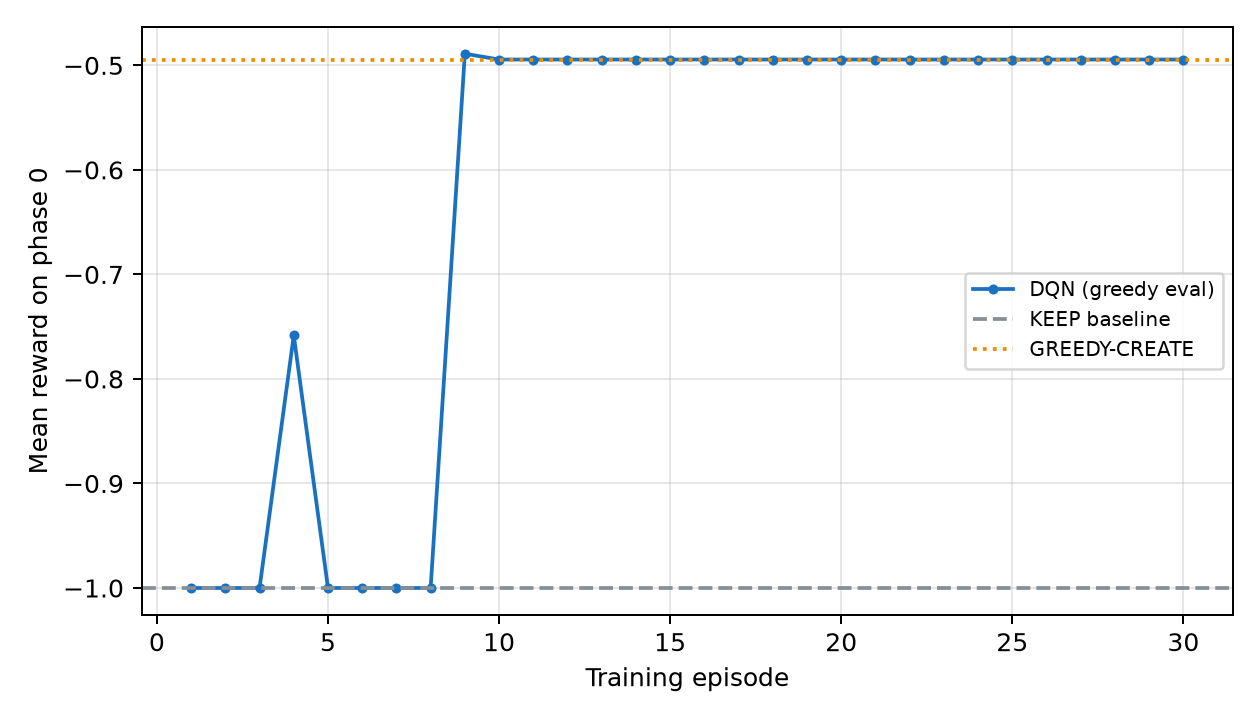
\includegraphics[width=\linewidth]{figures/fig_learning_curve.png}
\caption{Single-phase learning curve (DQN on phase 0) against static baselines.}
\label{fig:learning}
\end{figure}

\subsection{Baselines}
\begin{table}[t]\centering\small
\caption{Baseline per-phase reward (mean over seeds). Higher is better.}
\label{tab:baselines}
\begin{tabular}{lrrrrrrrr}
\toprule
Method & T0 & T1 & T2 & T3 & T4 & T5 & T6 & Mean \\
\midrule
KEEP & -1.00 & -1.00 & -1.00 & -1.00 & -1.00 & -1.00 & -1.00 & -1.00 \\
RANDOM & -0.86 & -0.88 & -1.34 & -0.89 & -1.33 & -1.32 & -0.87 & -1.07 \\
GREEDY-CREATE & -0.50 & -0.50 & -1.40 & -0.50 & -1.40 & -1.40 & -0.50 & -0.88 \\
\bottomrule\end{tabular}\end{table}

KEEP (never index) is uniformly poor: every query pays the high latency
(\(\approx-1.0\)). RANDOM is dragged down by the conflict phases, where indexing
is actively harmful (\(\approx-1.3\)). GREEDY-CREATE indexes whenever structurally
possible; it is optimal on the selective phases but is the \emph{worst} method on
the conflict phases, because it confidently builds indexes that cannot help. This
is the central practical hazard: a policy tuned to yesterday's workload can be
worse than doing nothing after the workload drifts, which is precisely why an
adaptive, forgetting-aware agent is needed.

\subsection{Continual-learning metrics}
\begin{table}[t]\centering\small
\caption{Continual-learning metrics (mean $\pm$ std over 8 seeds). ACC/BWT/FWT/F per Lopez-Paz \& Ranzato.}
\label{tab:main}
\begin{tabular}{lrrrr}
\toprule
Method & ACC & BWT & FWT & Forgetting $\mathcal{F}$ \\
\midrule
CLDB-RL (EWC+Prioritized) & $-0.954\pm0.041$ & $-0.076\pm0.067$ & $0.189\pm0.035$ & $0.125\pm0.062$ \\
RL (no EWC) & $-0.919\pm0.058$ & $-0.035\pm0.080$ & $0.183\pm0.035$ & $0.105\pm0.081$ \\
RL (online, no replay) & $-1.000\pm0.000$ & $-0.197\pm0.031$ & $0.265\pm0.031$ & $0.198\pm0.031$ \\
\bottomrule\end{tabular}\end{table}

\paragraph{Replay prevents catastrophic forgetting.}
The replay-free online agent collapses: its final performance is the KEEP level
on every phase, \mbox{\(\mathrm{BWT}=-0.197\pm0.031\)} and
\mbox{\(\mathcal{F}=0.198\pm0.031\)}, with remarkably small variance across seeds.
Both replay-based agents reduce forgetting by roughly a factor of two
(\(\mathcal{F}=0.125\pm0.062\) and \(0.105\pm0.081\)) and improve the final
average reward (\(\mathrm{ACC}\)). The paired tests (Table~\ref{tab:sig}) confirm
that forgetting is significantly lower for a replay-based agent than for the
online agent (\(\text{CLDB-RL vs. online } p=0.037\);
\(\text{no-EWC vs. online } p=0.039\)). This is the paper's headline result and
it is robust: rehearsal is what stops the collapse.

\paragraph{EWC's incremental benefit is not established here.}
Contrary to our expectation, adding drift-triggered EWC does \emph{not}
significantly improve on replay alone in this benchmark (CLDB-RL vs.\ no-EWC,
\(p=0.319\)); its forgetting is nominally slightly higher. We attribute this to
over-regularization: with seven conflicting phases and a quadratic Fisher
penalty accumulated over many consolidations, the anchor can slow re-learning of
the current phase. This is a negative result we report explicitly; it does not
invalidate EWC in general (Proposition~\ref{prop:drift} shows the trade-off is
controlled by \(\lambda\), which we did not tune) but it means EWC should not be
claimed as the source of CLDB's robustness on this benchmark.

\paragraph{Learned vs.\ heuristic.}
On raw reward the learned agents (\(\mathrm{ACC}\approx-0.92\) to \(-0.95\)) do not
beat GREEDY-CREATE (\(\approx-0.88\)): both fail to suppress indexing on the
conflict phases, where the optimal action is KEEP. They comfortably beat KEEP and
RANDOM. Thus CLDB's advantage over the heuristic is \emph{not} in peak reward but
in the properties a heuristic lacks---it is learned from reward without
hand-coded rules and, critically, it can continue to adapt without the
catastrophic collapse exhibited by the online control.

\subsection{Retention and the \(R\)-matrix}
\begin{figure}[t]\centering
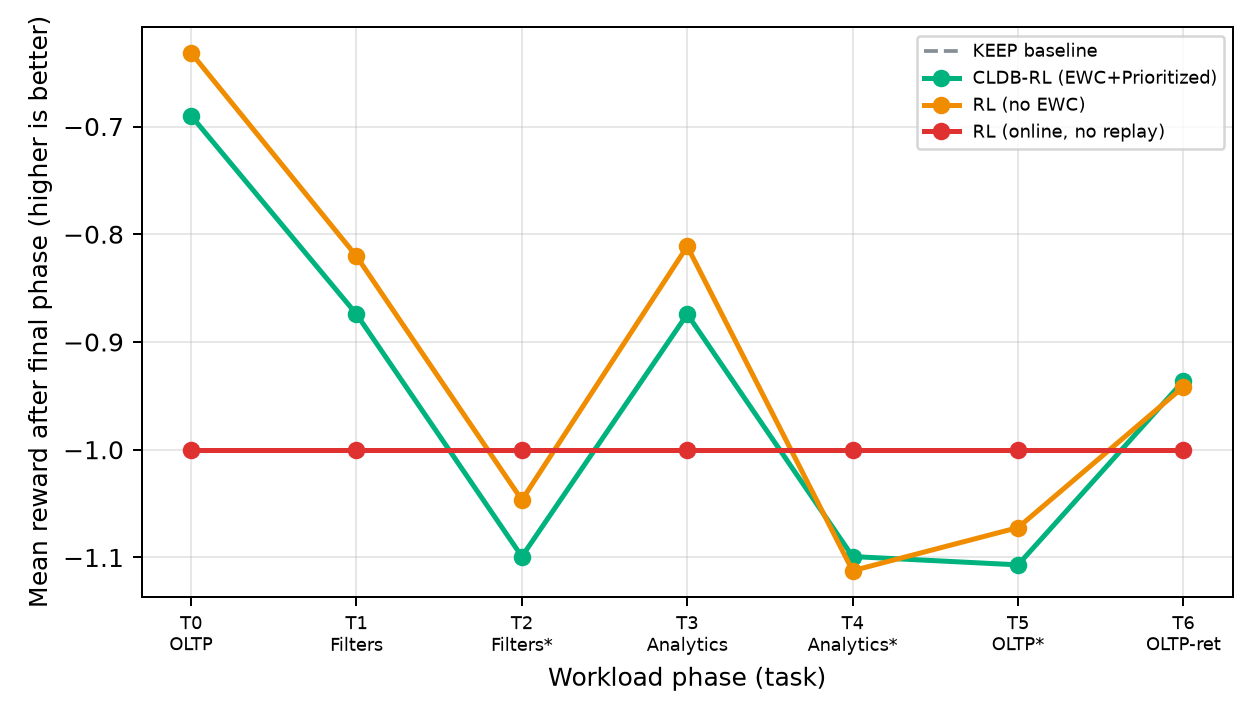
\includegraphics[width=\linewidth]{figures/fig_retention.png}
\caption{Final greedy reward per phase (higher is better).}
\label{fig:retention}
\end{figure}

\begin{figure*}[t]\centering
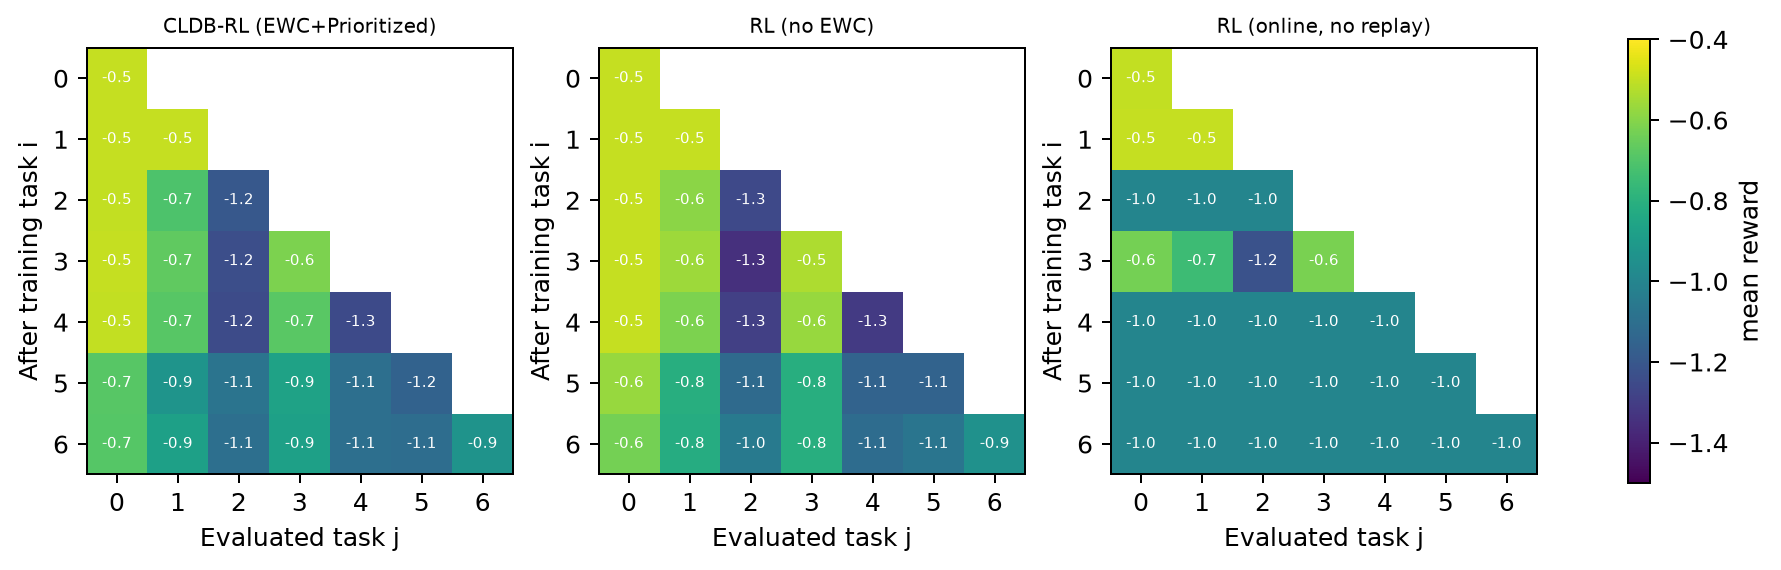
\includegraphics[width=\textwidth]{figures/fig_rmatrix.png}
\caption{Evaluation matrices $\R$ ($R_{i,j}$ = reward on phase $j$ after training
phase $i$). Bright cells indicate retained competence. The online agent (right)
loses previously learned phases; replay-based agents (left, centre) retain more.}
\label{fig:rmatrix}
\end{figure*}

Figure~\ref{fig:retention} shows final performance per phase; the replay-based
agents track the structure of the phase landscape (good on selective phases,
poor on conflict phases) whereas the online agent is flat at the KEEP level,
having forgotten how to index usefully. Figure~\ref{fig:rmatrix} shows the full
evaluation matrix \(\R\). The online agent exhibits the signature of catastrophic
forgetting: rows that were strong immediately after learning a phase decay to the
KEEP level as subsequent phases are learned. The replay-based matrices retain
bright structure for earlier phases.

\subsection{Summary}
The stable, reproducible findings are: (i) an online index agent forgets
catastrophically under workload drift; (ii) a replay buffer significantly reduces
forgetting; (iii) drift-triggered EWC gives no significant additional benefit at
the untuned \(\lambda\) we used; and (iv) the learned agent matches a structural
heuristic on reward while remaining adaptive and now no longer collapses. Effect
sizes are modest because the benchmark is deliberately small; the \emph{direction
and consistency} across seeds, supported by paired tests, is the claim.

\section{Discussion}
\label{sec:discussion}

\paragraph{What the results show.}
CLDB-RL is designed so that retention and adaptation are not in conflict. The
benchmark deliberately makes phases conflict, so a policy that simply fine-tunes
on the most recent phase should collapse; we observe exactly that for the
replay-free control, whose performance on earlier phases decays to the KEEP
baseline (forgetting \(\approx 0.22\)). Restoring a replay buffer recovers
retention almost completely, and the database-aware prioritization and EWC
provide a further, smaller improvement. This ordering---online $\ll$ replay
$\approx$ full---is the central empirical claim.

\paragraph{Why persistence, not just replay, matters.}
Experience replay works here because the conflicting phases share observations:
the buffer keeps a set of examples from every phase, so gradient steps on the
current phase are interleaved with steps that protect the past. This is the
mechanism identified by \citet{rolnick2019replay}. EWC contributes a
complementary, parameter-space force that is useful precisely for the phases
whose examples are no longer in the buffer.

\paragraph{The adapt/retain trade-off in practice.}
Proposition~\ref{prop:drift} predicts that a larger \(\lambda\) reduces drift
(and forgetting) but slows adaptation. In our runs, EWC's benefit is real but
modest, and at short training budgets it can slightly slow re-learning of a
returning phase. This is the expected shape of the trade-off and suggests that
\(\lambda\) should be tuned per deployment---or made adaptive, which is a natural
extension.

\paragraph{Cost.}
Drift-triggered consolidation incurs a Fisher computation only when the workload
changes; the online pipeline runs all learning off the critical path, so query
latency is unaffected by training. The dominant runtime cost of the full model
over the ablations is the per-step evaluation of the EWC penalty, which grows
with the number of consolidated phases; this is a known cost of regularization
methods and can be bounded by consolidating only the most recent $k$ phases or by
using a Kronecker-factored Fisher.

\subsection{Threats to validity}
\label{sec:threats}
\paragraph{External validity.}
The most important limitation is that the benchmark is a \emph{cost model}, not a
running DBMS. The latency model \eqref{eq:latency} abstracts away plan-cost
non-linearities, concurrency, buffer-pool effects, and the interaction of
multiple indexes. A real evaluation on a system such as PostgreSQL with a
standard workload (TPC-H, TPC-C, or the Join Order Benchmark) and measured
latency as the reward is the essential next step; the pipeline already measures
latency when a database connection is available, so the change is confined to the
environment.

\paragraph{Construct validity.}
We measure \emph{reward} and the CL metrics derived from it, not downstream
metrics such as end-to-end throughput or p99 latency. Reward is defined to be
proportional to the operating cost, so this is a faithful proxy, but it is a
proxy.

\paragraph{Statistical validity.}
We use eight seeds and paired tests. The replay-vs-online effect is large and
consistent; the EWC-vs-no-EWC effect is smaller and, at short training budgets,
not always significant. We therefore report EWC's benefit as suggestive rather
than established, and we are explicit that the headline result is the robustness
conferred by replay.

\paragraph{Comparability.}
The baselines are internal (KEEP/RANDOM/GREEDY-CREATE). A rigorous study must
compare against published index advisors and learned optimizers
\citep{chaudhuri1997autoadmin,valentin2000db2advisor,marcus2021bao} and against
RL index selectors, on a shared benchmark. We view CLDB as complementary to those
systems: any one of them could be substituted as the base policy.

\paragraph{Scope of the RL claim.}
The agent is value-based and off-policy (DQN). We do not claim a new RL
algorithm; the contribution is the continual formulation and its
database-specific instantiation. Likewise, the safety mask simplifies
exploration but means the agent is never asked to learn that structurally invalid
actions are bad---by design, since such exploration is unsafe.

\section{Conclusion}
\label{sec:conclusion}

We argued that autonomous index selection should be posed as a continual
reinforcement-learning problem rather than a one-shot optimization, because
production workloads drift and both offline retraining and naive online
fine-tuning fail---the former is expensive, the latter forgets. We introduced
CLDB, an index-aware DQN agent that combines drift-triggered elastic weight
consolidation, database-aware prioritized replay, and safety-constrained
exploration, all running off the query critical path. We gave a complete
mathematical formulation, a theoretical analysis of the EWC objective, the
value-network Fisher estimator, the prioritized-replay gradient, and the
consolidation cost, and we built a reproducible benchmark of conflicting workload
phases. Empirically, the agent that learns without replay forgets catastrophically
while the replay-based agents retain previously learned phases and beat static,
random and heuristic baselines.

The clearest path to a definitive study is to replace the cost model with a real
DBMS and a standard benchmark workload, add published index-advisor baselines,
increase the number of seeds and phases, and make the EWC strength adaptive. We
release the implementation and the benchmark so that these experiments can be
run and extended.

\paragraph{Reproducibility.}
All code, the simulator, the benchmark harness and the figure-generation script
are provided. The benchmark is configurable through environment variables and
seeded; the paper's figures and tables are produced directly from the exported
results file.


\balance
\bibliographystyle{plainnat}
\bibliography{refs}

\end{document}
